\documentclass[1pt, a4paper]{article}

%Texte et LuaLaTeX
\usepackage{luatextra}
\usepackage{polyglossia}
\setmainfont{Libertinus Serif}
% \setmainfont{Arial}
\usepackage[locale=FR]{siunitx}
\usepackage{booktabs}
\usepackage{xspace}
\usepackage{pict2e}
\usepackage{fullpage}
\usepackage{eso-pic}

\setlength{\unitlength}{1cm}

%Paramètres de langue
\setdefaultlanguage{english}
\setotherlanguage{french}

% Marges du document
\usepackage[lmargin=3cm, rmargin=2cm, vmargin=2.5cm]{geometry}

% En-tête et pieds de page
\iffalse
\usepackage{fancyhdr}
\pagestyle{fancy}
\fancyhead[R]{\textsc{sous-titre}}
\fancyhead[L]{Paradis Enzo}
\renewcommand{\footrulewidth}{1pt}
\fancyfoot[L]{catégorie}
\fancyfoot[R]{\thepage}
\fancyfoot[C]{}
\setlength{\headheight}{15pt}
\fi

%Packages maths
\usepackage{amsmath,amsfonts,amssymb,amsthm}
\usepackage{unicode-math}
%Autres
\usepackage{graphicx} %Insertion d'images
\usepackage{array}    %mise en forme tableau
\usepackage{hyperref} %liens internes au document
\usepackage{lipsum}   %lipsum
\usepackage{caption}  %caption sans figure
\usepackage{xcolor}
\usepackage{enumitem}
\usepackage{multicol}
\usepackage{subcaption}
\usepackage{tikz}
\usepackage{bbold}
\usepackage{appendix}
\usepackage{booktabs}
%code
\usepackage{minted}

%Optimisation
\renewcommand{\arraystretch}{1.2}
\renewcommand{\thesection}{\Roman{section}}

\numberwithin{equation}{section} 

\newcommand{\HRule}{\rule{\linewidth}{0.5mm}}
\newcommand{\blap}[1]{\vbox to 0pt{#1\vss}}
\newcommand{\tabitem}{~~\llap{\textbullet}~~}

\newcommand\PlaceFigure[3]{%
  \put(\LenToUnit{\dimexpr\paperwidth-#1},\LenToUnit{\dimexpr\paperheight-#2}){\blap{\llap{#3}}}%
}

\newcommand{\maketitlepage}{
\begin{titlepage}

% Add figure to titlepage
%   \AddToShipoutPicture{
%     }
 
    \begin{center}
        \huge\textbf{The Kuramoto Model}\\
        \large\textbf{Technical report for python numerical project}\\
        \vspace*{0.5cm}
        \large{Paradis Enzo}\\
        Student at the university of Bourgogne Franche-Comté\\
        Master CompuPhys - $1^{st}$ year\\
        \vspace*{1cm}
% You can add text here

    \end{center}
  
 
\end{titlepage}
\ClearShipoutPicture
\newpage}

\DeclareMathOperator{\e}{e}
\renewcommand{\exp}[1]{\e^{#1}}
\renewcommand{\vec}[1]{\overrightarrow{#1}}
\newcommand{\deriv}[1]{\mathrm{d}#1\\}
\newcommand{\moy}[1]{\ensuremath{\langle\;#1\;\rangle}\xspace}
\newcommand{\real}{\mathbb{R}}
\newcommand{\intg}{\mathbb{N}}
\newcommand{\oone}{\mathbb{1}}
\newcommand{\Ha}{\mathcal{H}}
\newcommand{\colVec}[4]{
    \begin{pmatrix} 
      #1\\ 
      #2\\
      #3\\
      #4
    \end{pmatrix}}
\newcommand{\rawVec}[4]{
    \begin{pmatrix} 
      #1 & #2 & #3 & #4
    \end{pmatrix}}
\newcommand*{\calVec}[4]{ 
    \left\lvert
      \begin{matrix} 
        #1\\
        #2\\
        #3\\
        #4
      \end{matrix}  
    \right.
  }
\newcommand{\derive}[2]{\dfrac{\deriv{#1}}{\deriv{#2}}}
\newcommand{\partd}[2]{\dfrac{\partial #1}{\partial #2}}
\newcommand{\ket}[1]{\ensuremath{|#1\rangle}\xspace}
\newcommand{\bra}[1]{\ensuremath{\langle #1|}\xspace}
\newcommand{\braket}[2]{\ensuremath{\langle #1 | #2 \rangle}\xspace}
\newcommand{\Braket}[3]{\ensuremath{\bra{#1}#2\ket{#3}}\xspace}
\newcommand{\abs}[1]{\ensuremath{\left|#1\right|}\xspace}
  %
\definecolor{couleur_lien}{RGB}{0, 102, 204}
\definecolor{couleur_lien2}{RGB}{0, 0, 254}
\hypersetup{
	colorlinks=true,
    linkcolor={couleur_lien2},
    citecolor={couleur_lien2},
    urlcolor={couleur_lien2}}

\unimathsetup{math-style=TeX}
\setmathfont{Libertinus Math}




\begin{document}
\maketitlepage
\tableofcontents
\newpage
\noindent
\section{Description of the main functions}
\noindent
All the functions which are used for the computing or the displaying of the results are called in the main file. At first there are the functions wich create the initial values in respect of the parameters set in the settings file, then this values are stocked in data (.dat) files in a directory named "parameters". With these data files, we don't have to repeat the calculations every time we want to test something. Then you have the functions that compute the results (the phase of the oscillators, the complex mean average, and the Shannon entropy), wich are stocked in data files in the same directory. And finally there are the functions that display the graphs by using the module \py{matplotlib.pyplot}. In this section we will describe the functions that create the datas files and their datas. Firstly the initial datas are created throught the \py{class Data} wich is in the data file. Finally the computing of the other values is in the \py{class KuramotoModel} wich is in the kuramoto file.
\subsection{The initialisation of the datas}
The initial datas are created by the function: \py{data.init_data(state)}:  
\begin{table}[htbp]
    \begin{center}
        \begin{tabular}{p{0.3\linewidth} p{0.3\linewidth} p{0.3\linewidth}} \toprule
            \multicolumn{3}{c}{\py{data.init_data(state="random")}}\\
            \midrule
            \hfil Description & \hfil Input & \hfil Output\\
            \cmidrule(r){1-1} \cmidrule{2-2} \cmidrule(l){3-3}
           
            This function is using to create initial values, stocked in data files in the directory parameters, according to the value of the argument \py{state} set by default to \py{state="random"}. You can create data for random, chimera, inverse, or josephson states. &
            The argument \py{state} is a \py{string}. By default it takes the value \py{"random"} but you can give it these values:\begin{itemize}
            \setlength{\itemsep}{0pt}
            \item \py{"random"}
            \item \py{"chimera"}
            \item \py{"inverse"}
            \item \py{"josephson"}
            \end{itemize}
            & This function will retrieve you six data file in the parameters directory, computing in according to the \py{state} argument.
            The data files are: \begin{itemize}
            \setlength{\itemsep}{0pt}
            \item \py{"omega.dat"}
            \item \py{"theta0.dat"}
            \item \py{"K.dat"}
            \item \py{"eta.dat"}
            \item \py{"alpha.dat"}
            \item \py{"tau.dat"}
            \end{itemize}\\
            \bottomrule
        \end{tabular}
    \end{center}
    \caption{function data.init\_data()}
    \label{tab:init_data}
\end{table}\\
Each \py{state} create six variables, wich are defined as follows:\\
The function \py{uniform()} is from the module \py{random}, and provide random numbers with uniform distribution, in the range given.
\begin{table}[htbp]
    \begin{center}
        \begin{tabular}{p{0.40\linewidth} p{0.40\linewidth}} \toprule
            \hfil \py{"random"} & \hfil \py{"chimera"}\\
            \cmidrule(r){1-1} \cmidrule(l){2-2}
            This \py{state} represent the case with random values defined by:
            \begin{itemize}
            \setlength{\itemsep}{0pt}
                \item $\omega^i=uniform(0, 3)$
                \item $\theta_0^i=uniform(0, \dfrac{2}{\pi})$
                \item $K^i_j=uniform(0, 1e10)$
                \item $\eta^i_j=uniform(0, 0.5)$
                \item $\alpha^i_j=uniform(0, \dfrac{2}{\pi})$
                \item $\tau^i_j=uniform(0, N//2)$
            \end{itemize}
            &This \py{state} represent the case for quantum chimera states defined by:
            \begin{itemize}
            \setlength{\itemsep}{0pt}
               \item $\omega^i=0.2 + i * 0.4 * sin(\dfrac{i^2 * \pi}{(2 * N^2)})$
               \item $\theta_0^i=uniform(0, \dfrac{2}{\pi})$
               \item $K^i_j=uniform(0, 1e10)\;if\;\abs{i-j}\leq M$
               \item $\eta^i_j=uniform(0, 0.5)$
               \item $\alpha^i_j=1.46$
               \item $\tau^i_j=uniform(0, N//2)$
            \end{itemize}\\
            \bottomrule
        \end{tabular}
    \end{center}
    \label{tab:states1}
\end{table}
\begin{table}[htbp]
    \begin{center}
        \begin{tabular}{p{0.40\linewidth} p{0.40\linewidth}} \toprule
            \hfil \py{"inverse"} & \hfil \py{"josephson"}\\
            \cmidrule(r){1-1} \cmidrule(l){2-2}
            This \py{state} represent the case with random values defined by:
            \begin{itemize}
            \setlength{\itemsep}{0pt}
                \item $\omega^i=0$
                \item $\theta_0^i=uniform(0, \dfrac{2}{\pi})$
                \item \begin{equation*}
                K^i_j=\left\{\begin{array}{ll}
                    \dfrac{1}{\abs{i-j}}\;if\;\abs{i-j}\leq M\;and\;\abs{i-j} \neq 0\\
                    1e20\;otherwise
                \end{array}\right.
            \end{equation*}
                \item $\eta^i_j=uniform(0, 0.5)$
                \item $\alpha^i_j=1.46)$
                \item $\tau^i_j=\abs{i-j}$
            \end{itemize}
            &This \py{state} represent the case for quantum chimera states defined by:
            \begin{itemize}
            \setlength{\itemsep}{0pt}
               \item $\omega^i=0.2 + i * 0.4 * sin(\dfrac{i^2 * \pi}{(2 * N^2)})$
               \item $\theta_0^i=uniform(0, \dfrac{2}{\pi})$
               \item $K^i_j=uniform(0, 1e10)\;if\;\abs{i-j}\leq M$
               \item $\eta^i_j=uniform(0, 0.5)$
               \item $\alpha^i_j=1.46$
               \item $\tau^i_j=uniform(0, N//2)$
            \end{itemize}\\
            \bottomrule
        \end{tabular}
    \end{center}
    \caption{\py{states}}
    \label{tab:states1}
\end{table}\\
\noindent
For each \py{state} choosen you have to define in the settings file the parameters \py{Nr} and \py{Nc}, to define the geometry of the system. \py{Nr} define the number of rows and \py{Nc} the number of columms, so \py{N=Nr*Nc} is the number of oscillators that you have. For example if you choose \py{N=12} in the geometry \py{Nr=3, Nc=4}, you will have this configuration:\\
\begin{figure}[htbp]
    \centering
    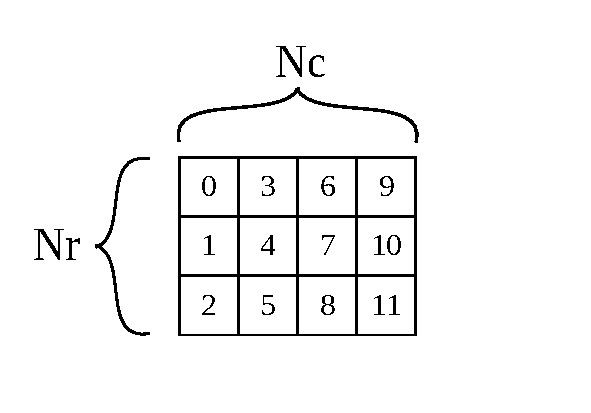
\includegraphics[scale=0.8]{figure/os_table.pdf}
    \caption{\py{Nr=3, Nc=4}}
    \label{fig:os_table}
\end{figure}\\
\noindent
If you put a non-positive number you will have some issues, the programm will not work. So be careful to respect the physics of the system.



\end{document}
